% =============================================================================
% Section 3: Composite Results
% =============================================================================
\section{Composite Results: Distribution, Ranking, and Classification
  Compression}\label{sec:composite-results}

\subsection{Summary statistics}

\Cref{tab:summary-stats} reports the distributional summary of the
ISI composite across the 27~EU member states.

\begin{table}[htbp]
\centering
\caption{ISI composite: summary statistics, EU-27, 2024.}
\label{tab:summary-stats}
\begin{tabular}{@{}lS[table-format=1.8]@{}}
\toprule
\textbf{Statistic} & {\textbf{Value}} \\
\midrule
$N$                         & 27 \\
Minimum                     & 0.23567126 \\
Maximum                     & 0.51748148 \\
Range                       & 0.28181022 \\
Mean                        & 0.34439144 \\
Median (P50)                & 0.34027984 \\
Std.\ dev.\ (pop.)         & 0.06992188 \\
Std.\ dev.\ (sample)       & 0.07125384 \\
Coeff.\ of variation (pop.) & 0.20303651 \\
\bottomrule
\end{tabular}
\end{table}

The composite mean (\num{0.34439144}) slightly exceeds the median
(\num{0.34027984}), indicating a mild positive skew driven by Malta's
outlying score of \num{0.51748148}.  The coefficient of variation
(0.203) is relatively low, indicating that the composite scores are
compressed relative to the full unit-interval range.  The range
(\num{0.28181022}) occupies only 28.2\% of the theoretical $[0, 1]$
interval, and the standard deviation is approximately one-fifth of
the mean.  These statistics indicate that the ISI composite
differentiates countries along a relatively narrow band rather than
spanning the full theoretically available range.

\subsection{Percentiles}

\begin{table}[htbp]
\centering
\caption{ISI composite: selected percentiles.}
\label{tab:percentiles}
\begin{tabular}{@{}lS[table-format=1.8]@{}}
\toprule
\textbf{Percentile} & {\textbf{Value}} \\
\midrule
P5   & 0.23604347 \\
P10  & 0.25534441 \\
P25  & 0.29179051 \\
P50  & 0.34027984 \\
P75  & 0.39060669 \\
P90  & 0.42586650 \\
P95  & 0.47131816 \\
\bottomrule
\end{tabular}
\end{table}

The interquartile range (IQR = P75 $-$ P25 = \num{0.09881618})
spans approximately 9.9 percentage points of the unit interval.
The P10--P90 range is \num{0.17052209}, indicating that the central
80\% of the distribution occupies roughly 17 percentage points.
The P5--P95 range extends to \num{0.23527469}, still well within the
unit interval.  The narrowness of the distribution has direct
implications for the classification scheme discussed in
\cref{sec:compression-diagnostics}: when most countries cluster in
a band of roughly 20 percentage points, threshold-based classification
will inevitably concentrate the majority in a single tier.

\subsection{Composite distribution}\label{sec:composite-distribution}

\Cref{fig:histogram} presents a histogram of the composite scores.
The distribution is unimodal with its mode in the 0.30--0.35 bin.
A visible right tail is produced by Malta and Cyprus.

\begin{figure}[htbp]
\centering
% F01: Histogram of ISI composite scores
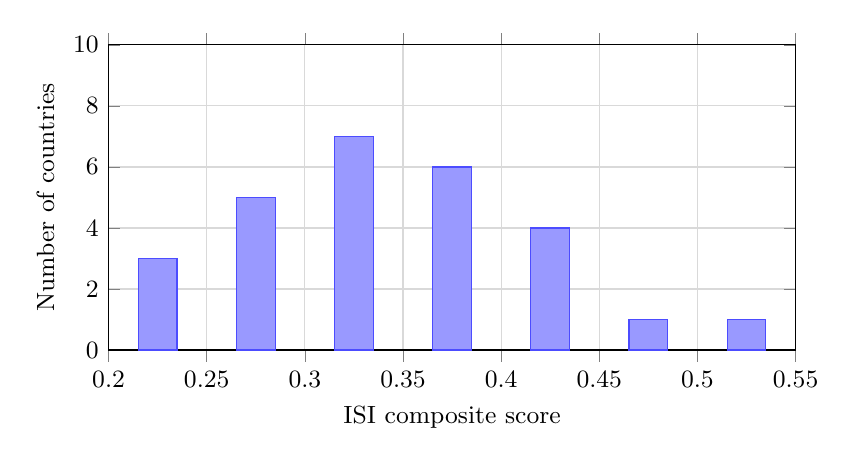
\begin{tikzpicture}
\begin{axis}[
  ybar,
  bar width=14pt,
  width=0.85\textwidth,
  height=0.45\textwidth,
  xlabel={ISI composite score},
  ylabel={Number of countries},
  xmin=0.20, xmax=0.55,
  ymin=0, ymax=10,
  xtick={0.20,0.25,0.30,0.35,0.40,0.45,0.50,0.55},
  ytick={0,2,4,6,8,10},
  grid=major,
  grid style={gray!30},
  tick label style={font=\small},
  label style={font=\small},
]
% Bin edges: 0.20-0.25, 0.25-0.30, 0.30-0.35, 0.35-0.40, 0.40-0.45, 0.45-0.50, 0.50-0.55
% Counts from data: [3, 5, 7, 6, 4, 1, 1]
\addplot[fill=blue!40, draw=blue!70] coordinates {
  (0.225, 3)
  (0.275, 5)
  (0.325, 7)
  (0.375, 6)
  (0.425, 4)
  (0.475, 1)
  (0.525, 1)
};
\end{axis}
\end{tikzpicture}

\caption{Histogram of ISI composite scores, EU-27, 2024.  Bin width
  = 0.05.  The dashed vertical line marks the population mean
  (\num{0.34439144}).}
\label{fig:histogram}
\end{figure}

\Cref{fig:ecdf} shows the empirical cumulative distribution function
(ECDF), which rises steeply between 0.26 and 0.42 and flattens at
the tails, consistent with the compressed mid-range clustering.

\begin{figure}[htbp]
\centering
% F02: ECDF of ISI composite scores
\begin{tikzpicture}
\begin{axis}[
  width=0.85\textwidth,
  height=0.50\textwidth,
  xlabel={ISI composite score},
  ylabel={Cumulative proportion},
  xmin=0.22, xmax=0.54,
  ymin=0, ymax=1.05,
  grid=major,
  grid style={gray!30},
  tick label style={font=\small},
  label style={font=\small},
  legend pos=south east,
  legend style={font=\footnotesize},
]
\addplot[blue!70, thick, const plot mark right] table[x index=0, y index=1]
  {tables/ecdf_coords.dat};
\addlegendentry{Empirical CDF}
% Reference line at mean
\draw[red, dashed, thin] (axis cs:0.33815860,0) -- (axis cs:0.33815860,1.05);
\node[red, font=\tiny, anchor=south west] at (axis cs:0.34,0.5) {Mean};
\end{axis}
\end{tikzpicture}

\caption{Empirical cumulative distribution function (ECDF) of ISI
  composite scores, EU-27, 2024.}
\label{fig:ecdf}
\end{figure}

The ECDF permits precise probability statements: approximately 50\%
of EU countries have composite scores between 0.29 and 0.40---a span
of only 11 percentage points.  The function is approximately
S-shaped, with steep inflection near the median and long, thin tails.
The lower tail contains only three countries (France, Slovakia,
Latvia) with scores below 0.25; the upper tail contains only Malta
above 0.50.

\subsection{Lorenz curve and Gini coefficient}

To further characterise the distribution, \cref{fig:lorenz} plots
the Lorenz curve of the composite scores (countries ordered from
lowest to highest ISI, cumulative share of total ISI on the vertical
axis).  The Gini coefficient is computed as:
\begin{equation}\label{eq:gini}
  G = 1 - 2\int_0^1 L(p)\,dp\,,
\end{equation}
where $L(p)$ is the Lorenz ordinate at population fraction $p$.

\begin{figure}[htbp]
\centering
% F03: Lorenz curve of ISI composite scores
\begin{tikzpicture}
\begin{axis}[
  width=0.65\textwidth,
  height=0.65\textwidth,
  xlabel={Cumulative share of countries},
  ylabel={Cumulative share of ISI composite},
  xmin=0, xmax=1,
  ymin=0, ymax=1,
  grid=major,
  grid style={gray!30},
  tick label style={font=\small},
  label style={font=\small},
  legend pos=north west,
  legend style={font=\footnotesize},
  axis equal image,
]
% 45-degree line of perfect equality
\addplot[gray, dashed, thin] coordinates {(0,0) (1,1)};
\addlegendentry{Perfect equality}
% Lorenz curve from data
\addplot[blue!70, thick] table[x index=0, y index=1]
  {tables/lorenz_coords.dat};
\addlegendentry{Lorenz curve (Gini = 0.1155)}
\end{axis}
\end{tikzpicture}

\caption{Lorenz curve of ISI composite scores, EU-27, 2024.
  Gini coefficient $= 0.1155$.  The diagonal represents perfect
  equality.}
\label{fig:lorenz}
\end{figure}

The Gini coefficient of \num{0.115463} indicates a relatively egalitarian
distribution.  For comparison, the Gini coefficient of GDP per capita
across EU countries typically ranges between 0.10 and 0.20, and the
Gini of income distributions within individual countries ranges from
0.25 to 0.40.  An ISI Gini of 0.115 places the cross-country
concentration distribution at the low end of cross-country inequality
measures, indicating that the EU-27 countries share broadly similar
levels of import concentration---albeit with substantial axis-level
heterogeneity, as demonstrated in subsequent sections.

\subsection{Full ranking}\label{sec:ranking}

\Cref{tab:ranking} presents the complete ranking of all 27~EU member
states.  Countries are ordered by descending composite score (rank~1
= most concentrated).

{\footnotesize
\setlength{\tabcolsep}{1pt}
\begin{longtable}{@{}r l S[table-format=1.8] S[table-format=1.8]
  S[table-format=1.8] S[table-format=1.8] S[table-format=1.8]
  S[table-format=1.8] S[table-format=1.8] l@{}}
  \caption{ISI composite and axis-level scores, EU-27, 2024.  Rank~1
    = most concentrated.}%
  \label{tab:ranking} \\
  \toprule
  {\textbf{Rk}} & {\textbf{Country}} & {\textbf{Comp.}}
    & {\textbf{Fin.}} & {\textbf{Ene.}} & {\textbf{Tech.}}
    & {\textbf{Def.}} & {\textbf{Crit.}} & {\textbf{Log.}}
    & {\textbf{Class.}} \\
  \midrule
  \endfirsthead
  \caption[]{ISI composite and axis-level scores (continued).} \\
  \toprule
  {\textbf{Rk}} & {\textbf{Country}} & {\textbf{Comp.}}
    & {\textbf{Fin.}} & {\textbf{Ene.}} & {\textbf{Tech.}}
    & {\textbf{Def.}} & {\textbf{Crit.}} & {\textbf{Log.}}
    & {\textbf{Class.}} \\
  \midrule
  \endhead
  \midrule
  \multicolumn{10}{r@{}}{\scriptsize\itshape Continued on next page} \\
  \endfoot
  \bottomrule
  \endlastfoot
  1  & Malta        & 0.51748148 & 0.13998786 & 0.35068126 & 0.20546991 & 1.00000000 & 0.40874987 & 1.00000000 & high.     \\
  2  & Cyprus       & 0.46821264 & 0.12407171 & 0.34768252 & 0.22438354 & 0.74847998 & 0.42359750 & 0.94106062 & mod.      \\
  3  & Ireland      & 0.42802519 & 0.14666620 & 0.46472525 & 0.58695939 & 0.44887460 & 0.30719544 & 0.61373023 & mod.      \\
  4  & Denmark      & 0.42442738 & 0.12401663 & 0.47029821 & 0.14995928 & 0.72368274 & 0.43629935 & 0.64230809 & mod.      \\
  5  & Croatia      & 0.40434768 & 0.27299265 & 0.35125471 & 0.17343982 & 0.74648317 & 0.52392772 & 0.35798800 & mod.      \\
  6  & Finland      & 0.40205136 & 0.11775073 & 0.36268783 & 0.19789321 & 0.38964518 & 0.54699996 & 0.79733123 & mod.      \\
  7  & Sweden       & 0.39871532 & 0.11646504 & 0.32721403 & 0.11982797 & 0.88107943 & 0.19257891 & 0.75512656 & mod.      \\
  8  & Austria      & 0.38249806 & 0.14903467 & 0.45581191 & 0.26057910 & 0.58506379 & 0.31857781 & 0.52592111 & mod.      \\
  9  & Italy        & 0.37386086 & 0.18753526 & 0.30781423 & 0.14103384 & 0.92057651 & 0.20839534 & 0.47781001 & mod.      \\
  10 & Slovenia     & 0.36979186 & 0.11917574 & 0.40540014 & 0.35739912 & 0.66661871 & 0.22301125 & 0.44714621 & mod.      \\
  11 & Greece       & 0.36537350 & 0.20078311 & 0.33541623 & 0.16272142 & 0.55148593 & 0.22200621 & 0.71982808 & mod.      \\
  12 & Luxembourg   & 0.36016893 & 0.11462818 & 0.35980871 & 0.20019721 & 0.64483831 & 0.22295831 & 0.61858285 & mod.      \\
  13 & Estonia      & 0.34332177 & 0.18172493 & 0.43935251 & 0.22713142 & 0.35561474 & 0.38622776 & 0.46987927 & mod.      \\
  14 & Bulgaria     & 0.34027984 & 0.16052965 & 0.35711773 & 0.15204272 & 0.86064518 & 0.14843767 & 0.36290606 & mod.      \\
  15 & Netherlands  & 0.33515702 & 0.12107826 & 0.31992851 & 0.12527375 & 0.95955396 & 0.13018835 & 0.35491930 & mod.      \\
  16 & Hungary      & 0.32966227 & 0.12222969 & 0.38580312 & 0.22538122 & 0.54471981 & 0.23405214 & 0.46578765 & mod.      \\
  17 & Portugal     & 0.32173430 & 0.18303606 & 0.34860414 & 0.19766062 & 0.43376254 & 0.25955617 & 0.50778629 & mod.      \\
  18 & Romania      & 0.31864192 & 0.20033340 & 0.40546401 & 0.29691153 & 0.56353195 & 0.15814280 & 0.28746783 & mod.      \\
  19 & Czechia      & 0.31796630 & 0.16116762 & 0.38082003 & 0.18242269 & 0.48413737 & 0.16976911 & 0.52948100 & mod.      \\
  20 & Poland       & 0.29561321 & 0.13314812 & 0.33487780 & 0.20845359 & 0.44326493 & 0.16532767 & 0.48860717 & mod.      \\
  21 & Belgium      & 0.28796781 & 0.15348744 & 0.30789144 & 0.29454573 & 0.44734854 & 0.17248330 & 0.35205038 & mod.      \\
  22 & Germany      & 0.26788694 & 0.10186464 & 0.32908790 & 0.09762824 & 0.58266751 & 0.22312039 & 0.27295297 & mod.      \\
  23 & Lithuania    & 0.26540520 & 0.13349636 & 0.33747627 & 0.24172279 & 0.40227798 & 0.13056067 & 0.34689716 & mod.      \\
  24 & Spain        & 0.26093977 & 0.14554195 & 0.30187479 & 0.19263249 & 0.38088569 & 0.11235234 & 0.43235135 & mod.      \\
  25 & Latvia       & 0.24695137 & 0.12316988 & 0.36522282 & 0.13309607 & 0.34079636 & 0.15120012 & 0.36822299 & mild      \\
  26 & Slovakia     & 0.23641567 & 0.16163673 & 0.39995460 & 0.21649186 & 0.00000000 & 0.15490434 & 0.48550648 & mild      \\
  27 & France       & 0.23567126 & 0.10039135 & 0.30911838 & 0.12001059 & 0.37034617 & 0.16122463 & 0.35293643 & mild      \\
\end{longtable}
}

Several features of the ranking are analytically significant.  First, the top two
positions are occupied by small island economies (Malta, Cyprus),
a pattern that aligns with the expectation that limited economic
scale and geographic isolation concentrate external dependencies.  Second, the
bottom three countries include two large economies (Germany rank~22,
France rank~27) and one small economy with anomalous defence data
(Slovakia rank~26).  Third, the mid-range (ranks 8--20) is
exceptionally compressed: the composite scores of Austria (rank~8,
\num{0.38249806}) and Poland (rank~20, \num{0.29561321}) differ by
only \num{0.08688485}, yet span 13~rank positions.  This compression
implies that small perturbations to the underlying data could produce
substantial rank reshuffling in the mid-range, a prediction confirmed
by the robustness exercises in \cref{sec:robustness}.

\subsection{Tier-compression analysis}

The classification distribution is highly compressed: 85.2\% of
countries fall in the moderately concentrated tier.  To quantify the
within-tier dispersion, \cref{tab:tier-compression} reports summary
statistics for each occupied tier.

\begin{table}[htbp]
\centering
\caption{Within-tier composite statistics.}
\label{tab:tier-compression}
\begin{tabular}{@{}lrS[table-format=1.8]S[table-format=1.8]S[table-format=1.8]S[table-format=1.8]@{}}
\toprule
\textbf{Tier} & {$n$} & {\textbf{Min}} & {\textbf{Max}} & {\textbf{Mean}}
  & {\textbf{Std (pop.)}} \\
\midrule
Highly concentrated & 1 & 0.51748148 & 0.51748148 & 0.51748148 & 0.00000000 \\
Moderately conc.    & 23 & 0.26093977 & 0.46821264 & 0.35327637 & 0.05339393 \\
Mildly concentrated & 3  & 0.23567126 & 0.24695137 & 0.24301277 & 0.00504709 \\
\bottomrule
\end{tabular}
\end{table}

Within the moderately concentrated tier, the range spans
\num{0.20727287} (from Spain at \num{0.26093977} to Cyprus at
\num{0.46821264}).  This wide within-tier range indicates that the
four-tier classification groups countries with meaningfully different
concentration profiles into the same category.  The tier structure is
informative at the extremes (Malta stands alone; the three mildly
concentrated countries cluster tightly) but provides limited
discriminatory power in the middle of the distribution.

\Cref{fig:rank-scatter} visualises the relationship between rank and
composite score, with horizontal colour bands indicating the tier
boundaries.

\begin{figure}[htbp]
\centering
% F_rank_scatter: Scatter plot of ISI composite vs rank
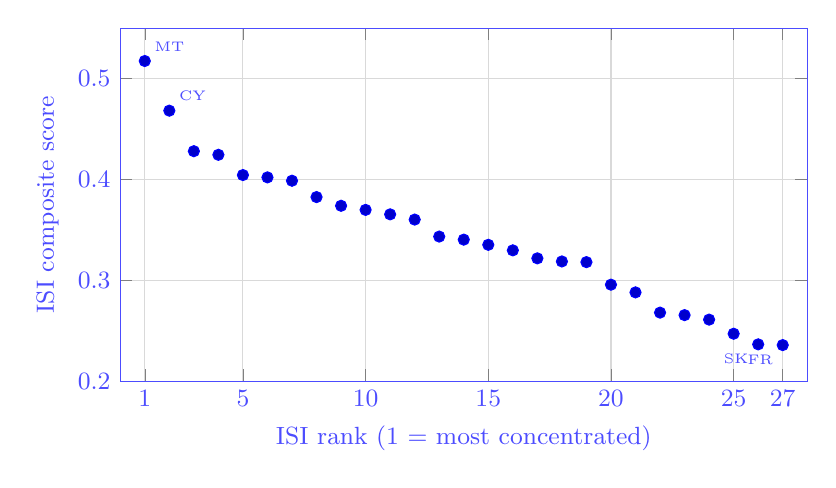
\begin{tikzpicture}
\begin{axis}[
  width=0.85\textwidth,
  height=0.50\textwidth,
  xlabel={ISI rank (1 = most concentrated)},
  ylabel={ISI composite score},
  xmin=0, xmax=28,
  ymin=0.20, ymax=0.55,
  xtick={1,5,10,15,20,25,27},
  grid=major,
  grid style={gray!30},
  tick label style={font=\small},
  label style={font=\small},
  only marks,
  mark=*,
  mark size=2pt,
  blue!70,
]
\addplot coordinates {
  (1, 0.51748148)
  (2, 0.46821264)
  (3, 0.42802519)
  (4, 0.42442738)
  (5, 0.40434768)
  (6, 0.40205136)
  (7, 0.39871532)
  (8, 0.38249806)
  (9, 0.37386086)
  (10, 0.36979186)
  (11, 0.36537350)
  (12, 0.36016893)
  (13, 0.34332177)
  (14, 0.34027984)
  (15, 0.33515702)
  (16, 0.32966227)
  (17, 0.32173430)
  (18, 0.31864192)
  (19, 0.31796630)
  (20, 0.29561321)
  (21, 0.28796781)
  (22, 0.26788694)
  (23, 0.26540520)
  (24, 0.26093977)
  (25, 0.24695137)
  (26, 0.23641567)
  (27, 0.23567126)
};
% Label extremes
\node[font=\tiny, anchor=south west] at (axis cs:1,0.5175) {MT};
\node[font=\tiny, anchor=south west] at (axis cs:2,0.4682) {CY};
\node[font=\tiny, anchor=north east] at (axis cs:27,0.2357) {FR};
\node[font=\tiny, anchor=north east] at (axis cs:26,0.2364) {SK};
\end{axis}
\end{tikzpicture}

\caption{Rank vs.\ ISI composite score with tier colour banding.
  The vertical axis shows the composite; horizontal position is
  the rank.  Colour bands: red ($\geq 0.50$, highly concentrated),
  amber ($[0.25, 0.50)$, moderately), green ($[0.15, 0.25)$, mildly).}
\label{fig:rank-scatter}
\end{figure}

\subsection{Classification compression diagnostics}\label{sec:compression-diagnostics}

The dominance of the moderately concentrated tier (23/27, 85.2\%)
raises the question of whether the four-tier classification scheme
provides adequate discriminatory power, or whether the observed
compression is an artefact of the threshold placement.  We address
this through three complementary diagnostics.

\subsubsection{Between-tier variance share ($\eta^2$)}

Let $\bar{x}_g$ denote the mean composite within tier~$g$ and
$\bar{x}$ the grand mean.  The between-tier sum of squares is
$SS_B = \sum_g n_g (\bar{x}_g - \bar{x})^2$, the within-tier sum of
squares is $SS_W = \sum_g \sum_{i \in g} (x_i - \bar{x}_g)^2$, and
the total is $SS_T = SS_B + SS_W$.  The $\eta^2$ statistic measures
the share of total variance explained by the tier assignment:
\begin{equation}\label{eq:eta-squared}
  \eta^2 = \frac{SS_B}{SS_T}\,.
\end{equation}

For the official ISI four-tier scheme applied to the EU-27 data:
\[
  SS_B = 0.06372\,,\quad
  SS_W = 0.06829\,,\quad
  SS_T = 0.13200\,,\quad
  \eta^2 = 0.483\,.
\]

An $\eta^2$ of 0.483 indicates that the tier classification captures
less than half of the total cross-country dispersion in composite
scores.  The within-tier variance ($SS_W$) slightly exceeds the
between-tier variance ($SS_B$), indicating that tier labels obscure
as much variation as they reveal.

\subsubsection{Comparison with data-driven alternatives}

\Cref{tab:compression-diagnostics} compares the official scheme with
two data-driven alternatives: terciles (three groups of approximately
equal size defined by the 33rd and 67th percentiles of the observed
distribution) and quartiles (four groups defined by the 25th, 50th,
and 75th percentiles).

% Table T15: Classification compression diagnostics
\begin{table}[htbp]
\centering
\caption{Classification compression diagnostics.  The official four-tier scheme
is compared with data-driven tercile and quartile alternatives.  $\eta^2 = SS_B / SS_T$
measures between-tier variance share.}
\label{tab:compression-diagnostics}
\small
\begin{tabular}{@{}l r S[table-format=1.8] S[table-format=1.10] l@{}}
\toprule
{\textbf{Tier}} & {$n$} & {\textbf{Mean}} & {\textbf{Var (within)}} & {\textbf{Scheme}} \\
\midrule
  Highly concentrated & 1 & 0.51748148 & 0.0000000000 & Official \\
  Moderately concentrated & 23 & 0.35052388 & 0.0029654931 & Official \\
  Mildly concentrated & 3 & 0.23967943 & 0.0000265329 & Official \\
\addlinespace
  T1 (low) & 9 & 0.26831306 & 0.0006888119 & Tercile \\
  T2 (mid) & 9 & 0.34268127 & 0.0003116324 & Tercile \\
  T3 (high) & 9 & 0.42218000 & 0.0018248593 & Tercile \\
\addlinespace
  Q1 (low) & 7 & 0.25731972 & 0.0003060842 & Quartile \\
  Q2 & 6 & 0.31979584 & 0.0001544247 & Quartile \\
  Q3 & 7 & 0.36218497 & 0.0002080999 & Quartile \\
  Q4 (high) & 7 & 0.43475158 & 0.0016297180 & Quartile \\
\midrule
  \multicolumn{5}{@{}l@{}}{$\eta^2$ (official) $= 0.482701$; Gini $= 0.115463$} \\
\bottomrule
\end{tabular}
\end{table}

The tercile boundaries fall at approximately 0.318 and 0.371, and the
quartile boundaries at approximately 0.292, 0.340, and 0.391.  Both
alternatives distribute countries more evenly across groups than the
official scheme, but at the cost of abandoning the structurally
motivated thresholds derived from HHI conventions.

\subsubsection{Interpretation}

The compression diagnostic establishes that the four-tier classification
is mathematically inevitable given the observed distribution.  The
composite distribution is unimodal and centred near 0.34, with most
of its mass in the $[0.26, 0.47]$ interval.  Any fixed-threshold
scheme with boundaries at 0.15, 0.25, and 0.50 will necessarily
concentrate the vast majority of countries in the tier spanning this
interval.  This is not a flaw in the classification but a consequence
of the empirical regularity that EU-27 countries exhibit similar
\emph{overall} concentration levels despite substantial heterogeneity
at the axis level.

The practical implication is that the tier label (``moderately
concentrated'') conveys limited information for the 23~countries in
that category.  For policy and analytical purposes, the full
composite ranking (\cref{tab:ranking}) and axis-level profiles
(\cref{sec:country-profiles}) provide far more discriminatory
information than the tier classification alone.
